\documentclass[a4paper,titlepage,report,disablejfam]{jsbook}

\usepackage[dvipdfmx]{graphicx}
\usepackage{emp} % 図の描画用
\usepackage[sc,slantedGreek]{mathpazo}
\usepackage{listings}
\usepackage{jlisting}
\usepackage{mathtools} % Ams-TeXの使用
\usepackage{mathrsfs} % 数式フォント
%\usepackage{MnSymbol} % 記号
\usepackage{amssymb,amsthm} % 記号と定理環境
\usepackage{proof} % 証明図
\usepackage{url} % URL
\usepackage{longtable} % 複数ページに亙る長い表
\usepackage{yhmath} % 長い括弧など
\usepackage{tablists}
%\usepackage[mathx]{mathabx}
\usepackage{stmaryrd}

% 定理類似環境:
\newtheorem{theo}{定理}
\newtheorem{defi}[theo]{定義}
\newtheorem{lemm}[theo]{補題}
\newtheorem{prop}[theo]{命題}
\renewcommand{\proofname}{\bf 証明}
\pagestyle{myheadings}

% 人名
\newcommand{\sakamoto}{酒本 典明}
\newcommand{\kobori}{小堀 育男}

% 見出し:
\renewcommand{\lstlistlistingname}{プログラム一覧}
\newsavebox{\articleauthor}
\newcommand{\responsibility}[1]{\nopagebreak[2]\begin{flushright}[文責: #1]\end{flushright}}
\newcommand{\defresponsible}[2]{\newenvironment{#1}[3][\relax]{%
\ifx##1\relax#2[##2 (##3)]{##2}%
\else#2[##1 (##3)]{##2}\fi%
\sbox{\articleauthor}{##3}}%
{\responsibility{\usebox{\articleauthor}}}}
\defresponsible{resbonsiblechapter}{\chapter}
\defresponsible{resbonsiblesection}{\section}

% 略語:
\newcommand{\algorithmW}{algorithm $\mathscr{W}$}
\newcommand{\algorithmU}{algorithm $\mathscr{U}$}

% 記号:
\DeclareSymbolFont{symbolsC}{U}{txsyc}{m}{n}
\DeclareMathSymbol{\strictif}{\mathrel}{symbolsC}{74}
\DeclareMathSymbol{\boxright}{\mathrel}{symbolsC}{128}
\newcommand{\R}{\mathbb{R}}
\newcommand{\Z}{\mathbb{Z}}
\newcommand{\N}{\mathbb{N}}
\newcommand{\msubset}{\subseteq}
\newcommand{\mnsubset}{\nsubseteq}
\newcommand{\mpsubset}{\subset}
\newcommand{\mnpsubset}{\nsubset}
\newcommand{\msupset}{\supseteq}
\newcommand{\mnsupset}{\nsupseteq}
\newcommand{\mpsupset}{\supset}
\newcommand{\mnpsupset}{\nsupset}
\newcommand{\limpl}{\supset}
\newcommand{\gtrdotrel}{\mathrel{\gtrdot}}
\newcommand{\Rrel}{\mathrel{R}}
\newcommand{\curlyveeord}{\mathord{\curlyvee}}
\newcommand{\curlywedgeord}{\mathord{\curlywedge}}

\newcommand{\powerset}{\mathfrak{P}}
\newcommand{\domain}{\mathop{\mathfrak{Dom}}}
\newcommand{\codomain}{\mathop{\mathfrak{Cod}}}

\newcommand{\mathnkop}[1]{\mathop{\mathsf{#1}}}
\newcommand{\mathnkenv}[1]{\mathcal{#1}}
\newcommand{\mathnkval}[1]{\mathsf{#1}}
\newcommand{\mathset}[1]{\mathit{#1}}
\newcommand{\mathfunc}[1]{\mathit{#1}}
\newcommand{\newmonadicopdot}[2]{\newcommand{#1}[2]{#2##1.\,##2}}
\newmonadicopdot{\foralldot}{\forall}
\newmonadicopdot{\existsdot}{\exists}
\newmonadicopdot{\lambdadot}{\lambda}
\newcommand{\fixdot}[2]{\mathnkop{fix}#1\;#2}
\newcommand{\fundot}[2]{\mathnkop{fun}#1\rightarrow#2}
\newcommand{\semanticS}[1]{\mathcal{S}\left\llbracket#1\right\rrbracket}
\newcommand{\semanticM}[1]{\mathcal{M}\left\llbracket#1\right\rrbracket}
\newcommand{\mypair}[2]{\left(#1,#2\right)}

\newcommand{\lambdaIf}{\mathop{\mathrm{if}}}
\newcommand{\lambdaThen}{\mathop{\mathrm{then}}}
\newcommand{\lambdaElse}{\mathop{\mathrm{else}}}
\newcommand{\lambdaLet}{\mathop{\mathrm{let}}}
\newcommand{\lambdaIn}{\mathop{\mathrm{in}}}

\newcommand{\semanticSVal}{\mathop{\pi_\mathrm{val}}}
\newcommand{\semanticSVEnv}{\mathop{\pi_\rho}}

\newcommand{\ltrue}{\top}
\newcommand{\lfalse}{\bot}
\newcommand{\defeq}{\triangleq} % 定義時に使う等号

\newcommand{\envExpr}{\mathnkenv{E}}
\newcommand{\envType}{\mathnkenv{T}}
\newcommand{\envVariant}{\mathnkenv{V}}
\newcommand{\envPattern}{{\mathnkenv{E}_p}}
\newcommand{\substExpr}{{\Sigma_\mathnkenv{E}}}
\newcommand{\substType}{{\Sigma_\mathnkenv{T}}}
\newcommand{\substVariant}{{\Sigma_\mathnkenv{V}}}
\newcommand{\applysubst}[2]{\mathfrak{S}\ #1\ #2}
\newcommand{\removeassoc}[2]{\mathfrak{Rm}\ #1\ #2}
\newcommand{\patternandenv}[2]{#1\Rsh#2}
\newcommand{\valueandenv}[2]{\mypair{#1}{#2}}
\newcommand{\domainrestrict}[2]{#1\mathbin{\upharpoonright}#2}
\newcommand{\freevars}[1]{\mathit{FV}(#1)}
\newcommand{\freetypevars}[1]{\mathit{FTV}(#1)}
\newcommand{\boundvars}[1]{\mathit{BV}(#1)}
\newcommand{\clauseor}{\mathbin{|}}
\newcommand{\patternor}{\mathbin{|}}
\newcommand{\patternand}{\mathbin{@}}
\newcommand{\patternany}{\_}

% 日本語特有の記号
\newcommand{\jpdash}{―\nobreak\hspace{-0.5zw}\nobreak―\nobreak\hspace{-0.5zw}\nobreak―}

\newcommand{\rulename}[1]{\text{\bfseries\scshape #1}}
\newcommand{\typename}[1]{\text{\sffamily\bfseries #1}}
\newcommand{\widevec}[1]{\overrightarrow{#1}}
\newcommand{\varrange}[1]{\boldsymbol{\widetilde{#1}}} %\widetriangle \widering \wideparen \widetilde \widehat のいづれかが良いと思う
\newcommand{\refEq}[1]{式\ref{#1}}
\newcommand{\refTbl}[1]{表\ref{#1}}
\newcommand{\refFig}[1]{図\ref{#1}}
\newcommand{\refCh}[1]{\ref{#1}章}
\newcommand{\refSc}[1]{\ref{#1}節}
\newcommand{\refSsc}[1]{\ref{#1}項}
\newcommand{\refSssc}[1]{\ref{#1}目}

% 罫線に太線を追加
\makeatletter
\def\@arrayrule{\@addtopreamble{%
\vrule \@width \arrayrulewidth}}
\def\Hline{\noalign{\hrule height 3\arrayrulewidth}}
%\def\LTHline{\noalign{\hrule height 3\arrayrulewidth}}
\def\Vline{\vrule width 3\arrayrulewidth}
%\def\LTHline{\LT@Hline}
\def\LT@Hline{%
  \noalign{\ifnum0=`}\fi
    \penalty\@M
    \futurelet\@let@token\LT@@Hline}
\def\LT@@Hline{%
  \ifx\@let@token\Hline
    \global\let\@gtempa\@gobble
    \gdef\LT@sep{\penalty-\@medpenalty\vskip\doublerulesep}%
  \else
    \global\let\@gtempa\@empty
    \gdef\LT@sep{\penalty-\@lowpenalty\vskip-\arrayrulewidth}%
  \fi
  \ifnum0=`{\fi}%
  \multispan\LT@cols
     \unskip\leaders\hrule\@height3\arrayrulewidth\hfill\cr
  \noalign{\LT@sep}%
  \multispan\LT@cols
     \unskip\leaders\hrule\@height3\arrayrulewidth\hfill\cr
  \noalign{\penalty\@M}%
  \@gtempa}
\def\LT@makecaption#1#2#3{%
  \LT@mcol\LT@cols c{\hbox to\z@%
  {\hss\parbox[t]\LTcapwidth{%
    \sbox\@tempboxa{#1{#2\hskip1zw\relax}#3}%
    \ifdim\wd\@tempboxa>\hsize
      #1{#2\hskip1zw\relax}#3%
    \else%
      \hbox to\hsize{\hfil\box\@tempboxa\hfil}%
    \fi%
    \endgraf\vskip\baselineskip}%
  \hss}}}%
\def\LT@array[#1]#2{%
  \refstepcounter{table}\stepcounter{LT@tables}%
  \if l#1%
    \LTleft\z@ \LTright\fill
  \else\if r#1%
    \LTleft\fill \LTright\z@
  \else\if c#1%
    \LTleft\fill \LTright\fill
  \fi\fi\fi
  \let\LT@mcol\multicolumn
  \let\LT@@tabarray\@tabarray
  \let\LT@@hl\hline
  \def\@tabarray{%
    \let\hline\LT@@hl
    \LT@@tabarray}%
  \let\\\LT@tabularcr\let\tabularnewline\\%
  \def\newpage{\noalign{\break}}%
  \def\pagebreak{\noalign{\ifnum`}=0\fi\@testopt{\LT@no@pgbk-}4}%
  \def\nopagebreak{\noalign{\ifnum`}=0\fi\@testopt\LT@no@pgbk4}%
  \let\hline\LT@hline \let\kill\LT@kill\let\caption\LT@caption
  \let\Hline\LT@Hline
% \@tempdima\ht\strutbox%                                       変更1
  \iftdir\@tempdima\ht\tstrutbox\else\@tempdima\ht\strutbox\fi%  <-
  \let\@endpbox\LT@endpbox
  \ifx\extrarowheight\@undefined
    \let\@acol\@tabacol
    \let\@classz\@tabclassz \let\@classiv\@tabclassiv
    \def\@startpbox{\vtop\LT@startpbox}%
    \let\@@startpbox\@startpbox
    \let\@@endpbox\@endpbox
    \let\LT@LL@FM@cr\@tabularcr
  \else
    \advance\@tempdima\extrarowheight
    \col@sep\tabcolsep
    \let\@startpbox\LT@startpbox\let\LT@LL@FM@cr\@arraycr
  \fi
  \setbox\@arstrutbox\hbox{\vrule
    \@height \arraystretch \@tempdima
%   \@depth \arraystretch \dp \strutbox%          変更2
    \iftdir\@depth \arraystretch \dp \tstrutbox%   <-
    \else\@depth \arraystretch \dp \strutbox\fi%   <-
    \@width \z@}%
  \let\@sharp##\let\protect\relax
   \begingroup
    \@mkpream{#2}%
    \xdef\LT@bchunk{%
       \global\advance\c@LT@chunks\@ne
       \global\LT@rows\z@\setbox\z@\vbox\bgroup
       \LT@setprevdepth
       \tabskip\LTleft \noexpand\halign to\hsize\bgroup
      \tabskip\z@ \@arstrut \@preamble \tabskip\LTright \cr}%
  \endgroup
  \expandafter\LT@nofcols\LT@bchunk&\LT@nofcols
  \LT@make@row
% \m@th\let\par\@empty%                               変更3
  \iftdir\m@th\let\par\@@par%                          <-
  \else\m@th\let\par\@empty\fi%                        <-
  \everycr{}\lineskip\z@\baselineskip\z@
  \LT@bchunk}

\makeatother

% listings用設定
\lstdefinelanguage{nibkame}{%
   morekeywords={%
        let,letrec,if,match,with,type,fun,+,-,*,/,+.,-.,*.,\.,(),~-,;,
        and,or,not,unit,Nil%
   },%
%   morekeywords={%
%        ignore
%   },%
%   morekeywords={%
%        print_int,print_float,print_char,print_string
%   },%
%   morekeywords={%
%        hd,tl,null,map,length
%   },%
%   morekeywords={%
%        array-create,array-set,array-ref,array-from-list,array-from-list-with-length
%   },%
   sensitive,% ???
   alsodigit=->,%
   morecomment=[l];,%
   morecomment=[s]{\#|}{|\#},%
   morestring=[b]",%"
   literate=%
       {[|}{[\hskip -1pt$|$}2%
       {|]}{$|$\hskip -1pt]}2%
%      {[]}{\ensuremath{[\hskip -0.1em]}}2%
       {->}{\ensuremath{\rightarrow}~}2%
       {::}{\ensuremath{:\hskip -0.1em:}~}2%
}[keywords,comments,strings]

\lstdefinelanguage[Objective display]{Caml}[Objective]{Caml}{%
    morestring=[d]',%'
%    classoffset=2,
%    morekeywords={int,float,char,string},keywordstyle=\color{red},
%    classoffset=3,
%    morekeywords={list,array},keywordstyle=\color{blue},
%    classoffset=0,
    literate=%
        {[|}{[\hskip -1pt$|$}2%
        {|]}{$|$\hskip -1pt]}2%
%       {[]}{\ensuremath{[\hskip -0.1em]}}2%
        {->}{\ensuremath{\rightarrow}~}2%
        {::}{\ensuremath{:\hskip -0.1em:}~}2%
}
\lstset{%
  %language=[Objective display]Caml,%
  language=nibkame,%
  basicstyle={\normalfont\normalsize\sffamily},%
  commentstyle={\small\ttfamily\itshape\bfseries\upshape},%
  classoffset=1,%
  keywordstyle={\bfseries},%
  %frame=,%
  %framesep=0pt,%
  showstringspaces=false,%
  %numbers=left,%
  %numberstyle={\scriptsize},%
  %stepnumber=1,%
  tabsize=8,%
  lineskip=-0.5ex,%
%
  breaklines=true,%
  linewidth=\the\textwidth,
%  columns=[l]flexible%
  columns=flexible%
}


\begin{document}
\title{電子情報工学科実験報告書 \\ 関数型言語の設計と実装}
\author{
\begin{tabular}{llr}
 L班 & 07317 & 小堀 育男 \\
     & 07322 & 酒本 典明
\end{tabular}
}
\date{平成23年2月3日}

\frontmatter

\maketitle

\tableofcontents
%\listoffigures
%\listoftables
%\lstlistoflistings

\newpage

\mainmatter % 序論も本文の内

\chapter{序論}\label{ch:intro}
\begin{abstract}
 本実験課題選定の理由と目的について論じる.また,実装の概要と報告書の構成を述べる.
\end{abstract}

\begin{resbonsiblesection}{目的}{\kobori}
関数型言語の有用性はHughes\cite{hughes1989functional}などにより主張され
ていた.現在では,関数型言語に由来する機能が,C++やJava, C\# など
の言語に取り込まれている.またScala\footnote{\url{http://www.scala-lang.org/}}
やF\#{}\footnote{\url{http://msdn.microsoft.com/ja-jp/fsharp}}
など既存の手続き型言語との連携を強く意識した言語も登場している.

関数型言語に特徴的な機能として第一級の関数やクロージャなどがある.これら
は計算機の命令セットの持つ機能からかけ離れている.こういった機能を持った
言語を設計し,実装することで機能に対する理解を深めることを目標とする.

そのために,我々は静的に強く型付けされる関数型言語nibkameを設計しコンパ
イラを実装した.これは学生実験における参照実装として開発された
MinCaml\cite{住井英二郎:2008-04-24}を基にして開発を行なった.

MinCamlおよびMinCamlコンパイラは簡潔な実装(約2000行ほど)で性能の良いコー
ドを生成することに特徴のある関数型言語である.構文はObjective
Caml\footnote{\url{http://caml.inria.fr/ocaml/}}のサブセットであり,算術演算や
タプル構造,破壊的代入の可能な配列,高階関数,再帰と末尾呼び出し,型推論
などの機能が実現されており,レイトレーシングなどの複雑なプログラムを記述
することができる.MinCamlはプログラム言語処理系の教材として用いられるこ
とを主眼としており,その機能選定は実装を簡潔に保つことを重視して行われた.

簡潔さを保つために,多くのアプリケーションプログラムを記述するときに必須
でない機能は省略された.その中にはMinCamlコンパイラの記述に多く用いられ
ている代数的データ型やパターンマッチングなどが存在する.
nibkameではそういった機能と,その他にも生産性に高い影響を与える機能を追
加することでより実用的な言語を開発することを目指した.
MinCamlコンパイラはターゲットとする計算機としてSPARCとPowerPCをサポート
している.しかし実行する計算機の確保の容易さから,nibkameコンパイラはター
ゲットをIA-32アーキテクチャとした.

詳しくは\refCh{ch:lang_design}で述べるが,これらの目標を達成するために次
に挙げる機能の追加を行った.
\begin{itemize}
 \item トップレベル環境における複数の式
 \item 多相関数
 \item 代数的データ型
 \item パターンマッチング
 \item IA-32アーキテクチャ向け機械語の生成
\end{itemize}
また,これを達成するために,複数の定義をひとまとめに扱うモジュール機構と
3番地形式の中間言語の2番地形式への変換,メモリ管理機構の強化が必要となっ
た.
\end{resbonsiblesection}

\section{実装概要}
コンパイラの主要部分はObjective
Camlを用いて実装した.構文解析部分はScheme
(処理系としては
Gauche\footnote{\url{http://practical-scheme.net/gauche/index-j.html}})
を用いた.実行時ランタイムはC言語にて実装した.
% ここに行数などを含むといいみたい

2011年1月12日時点でのソースコードの全行数は7001行であり,
ソースソードの目的別言語別行数内訳は\refTbl{tbl:sourcecode-lines}のようになっている.

\begin{table}[hbt]
    \caption{ソースコードの行数}\label{tbl:sourcecode-lines}
    \begin{center}
    \begin{tabular}{cllr@{行}}
        \Hline
        \multicolumn{1}{c}{目的} & \multicolumn{2}{c}{言語} & \multicolumn{1}{c}{行数} \\
        \hline
        本体        & O'Caml & 実装             & 4820 \\
	                & O'Caml & インターフェース & 781 \\
	                & Scheme &                  & 337 \\
	                & C言語  &                  & 0 \\
        単体テスト  & O'Caml & 実装             & 1063 \\
        \Hline
    \end{tabular}
    \end{center}
\end{table}

\section{報告書の構成} % ここは内容にあわせて書き換えてください.あと
			  % subsectionはオーバースペックな気が.
\refCh{ch:preparation}ではコンパイラの動作を理解するために必要となる理論
や規則について概説する.本報告書で用いる論理学や集合の記法についても説明
する.
\refCh{ch:lang_design}では,nibkame言語に搭載された機能のうち関数型言語
に特有なものについて説明し,最終的に実装された言語機能と構文を示す.
\refCh{ch:impl}ではコンパイラのモジュール構造と各フェーズの対応を示し,
コンパイラの実装について説明する.
\refCh{ch:sample-program}では実際のnibkameプログラムの例を示し,コンパイラの動作
と得られる目的プログラムについて説明する.
\refCh{ch:conclude}では実装した機能についてまとめ,これからの課題を議論する.

%\mainmatter
%\chapter{原理}\label{ch:原理}

\chapter{準備}\label{ch:preparation}
\begin{abstract}
本報告書で用いる理論・記法について概説する. 
本章で説かれる内容は本報告書で用いられる範囲に限定し,
かつ,直感的な解りやすさを最優先としたため,
論理的に不正確な箇所が多々あるがお赦し願いたい.
\end{abstract}

\begin{resbonsiblesection}{全体的な記法について}{\sakamoto}\label{sc:about-notation}
以下,演算子の結合力を表す際に,
\begin{equation}\label{eq:bonding-strength}
\times \gtrdotrel +
\end{equation}
と表すこととする.
これは,$A\times B + C$という式があったときに$(A\times B)+ C$と解釈することを意味する.

等号系の記号の使い分けは\refTbl{tbl:equal-usage}のようにする.

\begin{table}[hbt]
    \caption{等号系記号の使い分け}\label{tbl:equal-usage}
    \begin{center}
    \begin{tabular}{cp{40zw}}
        \Hline
        \multicolumn{1}{c}{記号} & \multicolumn{1}{c}{目的} \\
        \hline
        $=$ & 通常の等値,即ち数値・真偽値・集合などの等しさを真偽値で表す,または,等しいことを言明する. \\
        $\equiv$ & $=$よりも広い意味で同じであることを表す. \\
        $\defeq$ & 通常の式において左辺の記号が右辺で定義されることを示す.\\
        $\Coloneqq$ & BNFにおいて,左辺の記号が右辺で定義されることを示す.\refSc{sc:about-BNF-form} \\
        \Hline
    \end{tabular}
    \end{center}
\end{table}

変数$e$の動く領域を$\varrange{e}$と表すこととする\footnote{一般的な方法ではない}.

自然数$\N$は0を含むこととする.
\end{resbonsiblesection}

\begin{resbonsiblesection}{集合について}{\sakamoto}\label{sc:about-set}
元として含むことを表す記号として$\in$,$\ni$を用いる.  部分集合を表す記号として$\msubset$,$\msupset$を,真部分集合を表す記号として$\mpsubset$,$\mpsupset$を用いる. 空集合の記号としては$\emptyset$を用いる.

集合$x$の羃集合は$\powerset x$若しくは$\powerset(x)$と書く
\footnote{$2^x$や$\boldsymbol{2}^x$という表記も一般的.}.

順序対若しくは単純に対は,$(x,y)$と表すことにする\footnote{標準的には$\left\langle x,y\right\rangle$である.}.
順序対は
\begin{equation}
(x_0,x_1) = (y_0,y_1) \iff x_0 = y_0 \land x_1 = y_1
\end{equation}
という式によって特徴付けられる.
組は$(x_0,x_1,\cdots,x_n)$と表すことにする\footnote{これも標準的には$\left\langle x_0,x_1,\cdots,x_n\right\rangle$である.}.
順序対と同様に
\begin{equation}
(x_0,x_1,\cdots,x_n) = (y_0,y_1,\cdots,x_n) \iff \foralldot{i\in\{0,1,\cdots,n\}}{x_i = y_i}
\end{equation}
となる.
$(x_0,x_1,\cdots,x_n)$は$(x_i)_{i\in\{0,1,\cdots,n\}}$とも書く.

積集合とはいくつかの集合の要素で組を作ったときの集合のことであり,
\begin{equation}
X_0\times X_1\times\cdots\times X_n\triangleq \{(x_0,x_1,\cdots,x_n)|\foralldot{i\in\{0,1,\cdots,n\}}{x_i\in X_i}\}
\end{equation}
と定義される.
$X_0\times X_1\times\cdots\times X_n$は$\prod_{i\in\{0,1,\cdots,n\}} X_i$とも書く.

標準射影$\pi_i:\left(\prod_{j\in\{0,1,\cdots,n\}} X_j\right)\rightarrow X_i$とは,組または対からその構成要素を取り出す演算であり,
\begin{equation}
\pi_i(X_0\times X_1\times\cdots\times X_n)\triangleq X_i
\end{equation}
である.

順序対の集合$X$\jpdash 例えば,$X=\{(x,y)|x\in\R,y\in\Z\}$など\jpdash は二項関係とも呼ばれ,
その始域$\domain X$,終域$\codomain X$は夫々,
\begin{align}
    \domain X &\triangleq \{\pi_0 x|x\in X\}\\
    \codomain X &\triangleq \{\pi_1 x|x\in X\}
\end{align}
と定義される.
二項関係$R$に対して,始域を集合$C$に限定した二項関係$\{x|x\in R, \pi_0 x\in C\}$を
$\domainrestrict{R}{C}$と書く.
二項関係への追加$R\uplus\mypair{x}{y}$は,
$R\uplus\mypair{x}{y}\triangleq \domainrestrict{R}{\left(\domain R\setminus \{x\}\right)}$
と定義される.

$x_0,x_1,\cdots,x_n$ ($n\in\N$)という並びをを$\vec{x}$と略記する.

\end{resbonsiblesection}

\begin{resbonsiblesection}{論理について}{\sakamoto}\label{sc:about-logic}
真・偽を表すの記号として夫々,$\ltrue$,$\lfalse$を用いる.
論理和・論理積・否定・含意の記号として夫々,$\lor$,$\land$,$\lnot$,$\limpl$を用いる.
変数$x$がその領域$\varrange{x}$を動くとき,
述語$P(x)$が全ての$x$で真になることを$\foralldot{x}{P(x)}$,
述語$P(x)$がある$x$で真になることを$\existsdot{x}{P(x)}$と表す.
$\foralldot{x}{\foralldot{y}{\cdots}}$は$\foralldot{x,y,\cdots}{}$と略記する.
$\exists$も同様.

$\forall$,$\exists$,$\lnot$,$\limpl$は右結合性,
例えば,$\lnot\lnot A\equiv \lnot(\lnot A)$,$A\limpl B\limpl C \equiv A\limpl (B\limpl C)$とする.
夫々の演算子の優先順位は$\lnot\gtrdotrel\land,\lor\gtrdotrel\limpl$となる.

\begin{equation}\label{eq:def-mp}
\infer[\rulename{M.P.}]{\beta}{\alpha & \alpha \limpl \beta}
\end{equation}
は,$\alpha$と$\alpha \limpl \beta$という仮定から,\rulename{M.P.}という推論規則によって$\beta$が導き出されることを表す記法である.
\ref{eq:def-mp}によって定義される推論規則は,推論規則内の$\alpha$,$\beta$に式を代入することによって
\begin{equation}\label{eq:def-mp-instance-1}
\infer[\rulename{M.P.}]{A\land B}{A & A \limpl A\land B}
\end{equation}
や,
\begin{equation}\label{eq:def-mp-instance-2}
\infer[\rulename{M.P.}]{\foralldot{x}{Q(a, x) \limpl P(x)}}{\existsdot{x}{P(x)} & \existsdot{x}{P(x)} \limpl \foralldot{x}{Q(a, x) \limpl P(x)}}
\end{equation}
も表す.
この例における$\alpha$,$\beta$のように,超文脈的に扱われる変数のことをメタ変数(meta-variable)と呼ぶ.


$\Gamma_1,\Gamma_2,\cdots\vdash A_1, A_2,\cdots$は,
主に,$\Gamma_1, \Gamma_2, \cdots$から$A_1, A_2, \cdots$が推論できることを表す記法として用いる.
\end{resbonsiblesection}

\begin{resbonsiblesection}{バッカス・ナウア記法について}{\sakamoto}\label{sc:about-BNF-form}
バッカス・ナウア記法(Backus-Naur Form, BNF)
は文脈自由文法を定義するのに用いられるメタ言語であって,
プログラミング言語の構文記述やデータ構造の記述など,広汎に利用される.
計算機科学でも式として頻繁に用いられるので解説する.

$\Coloneqq$の左辺にある名前は右辺にある式で定義される.
例えば,
\begin{equation}\label{eq:bnf-example-1} 
e\Coloneqq \mathsf{abc}
\end{equation}
というBNFに対しては
\begin{equation}
\varrange{e} = \{\mathsf{abc}\}
\end{equation}
となる.

右辺において$\mid$は「または」の意味を表し,$\mid$で区切られたいずれかの式に当てはまる.例えば,
\begin{equation}\label{eq:bnf-example-2} 
e\Coloneqq \mathsf{a} \mid \mathsf{b} \mid \mathsf{c}
\quad\text{または}\quad
\begin{array}{rcl}
    e    &\Coloneqq& \mathsf{a} \\
            &\mid&   \mathsf{b} \\
            &\mid&   \mathsf{c} 
\end{array}
\end{equation}
というBNFに対しては
\begin{equation}
\varrange{e} = \{\mathrm{a}, \mathrm{b}, \mathrm{c}\}
\end{equation}
となる.

右辺において左辺の記号が使われた場合は再帰となる
\begin{equation}\label{eq:bnf-example-3} 
\begin{array}{rcl}
    e    &\Coloneqq& \mathsf{a} \\
            &\mid&   e\mathsf{'} 
\end{array}
\end{equation}
というBNFに対しては
\begin{equation}
\varrange{e} = \{\mathrm{a}, \mathrm{a'}, \mathrm{a''}, \mathrm{a'''}, \cdots \}
\end{equation}
となる.
\end{resbonsiblesection}

\begin{resbonsiblesection}{ラムダ式について}{\sakamoto}\label{sc:about-lambda-expression}
ラムダ式(lambda expression,$\lambda$-expression) とは,一言で言ってしまうと関数そのものを抽象化したものである.

例えば以下の式を考えよう.
\begin{align}
f(x) &= (x + 1)^2\\
f(x + 1) &= {\left((x + 1) + 1\right)}^2 = x^2 + 4x + 4\\
(x + 1) &= x + 1
\end{align}
これは$(x + 1)$に対して関数$f$を適用すると$x^2 + 2x + 1$となるが,
関数を適用しないとそれは$x + 1$そのものであることを表している.

では逆に,$f$に引数を適用しないとどうなるのであろうか.
\begin{align}
f(x) &= x^2 + 2x + 1\\
f    &= \;?
\end{align}
この場合の$f$そのものを表すのにラムダ式を用いることが出来,そうすると
\begin{align}
f &= \lambdadot{x}{(x^2 + 2x + 1)}
\end{align}
となって関数そのものを陽に扱うことが出来る.
以下,必要の無い限り括弧は省略し,$\lambdadot{x}{(x^2 + 2x + 1)}$は$\lambdadot{x}{x^2 + 2x + 1}$と書く.

ラムダ式を用いて記述した関数に引数を適用させると,
\begin{align}
f(y) &= (\lambdadot{x}{x^2 + 2x + 1})(y) = y^2 + 2y + 2 \\
f(2) &= (\lambdadot{x}{x^2 + 2x + 1})(2) = 2^2 + 2\cdot 2 + 1 = 9
\end{align}
となる.

次に複数引数の関数を考えよう.
\begin{align}
g(x, y) &= x + y
\end{align}
この関数を表すためには,
$\lambdadot{x,y}{}$という記法を導入するのが良いと思われる.
従って,
\begin{align}
\label{eq:lambda-multiple}
g &= \lambdadot{x,y}{x + y}\\
\label{eq:lambda-multiple-inst}
g(a, b) &= a + b\\
g(1, 2) &= (\lambdadot{x,y}{x + y})(1, 2) = 1 + 2 = 3
\end{align}
と表せる.

ここで,天下り的ではあるが,$\lambdadot{x}{\lambdadot{y}{x+y}}$を考える.
すると,
\begin{gather}
\begin{aligned}
\label{eq:lambda-curried}
h &= \lambdadot{x}{\lambdadot{y}{x+y}} \\
\end{aligned} \\
\begin{aligned}
\label{eq:lambda-curried-partial}
h(a) &= (\lambdadot{x}{\lambdadot{y}{x+y}})(a)\\
     &= {\lambdadot{y}{a+y}}
\end{aligned} \\
\begin{aligned}
\label{eq:lambda-curried-inst}
\left(h(a)\right)(b) &= \left((\lambdadot{x}{\lambdadot{y}{x+y}})(a)\right)(b) \\
        &= (\lambdadot{y}{a+y})(b)\\
        &= a + b
\end{aligned} \\
\begin{aligned}
\left(h(1)\right)(2) &= \left((\lambdadot{x}{\lambdadot{y}{x+y}})(1)\right)(2) \\
        &= (\lambdadot{y}{1+y})(2) \\
        &= 1 + 2 = 3
\end{aligned}
\end{gather}
このようになる.
以下,$f(a)(b)(c)\cdots$は
$\delimitershortfall-1pt\left({\cdots\left({\left({\left({f(a)}\right)(b)}\right)(c)}\right)\cdots}\right)$
を表すものとし,
必要の無い限り括弧を省略する.

ここで,
\refEq{eq:lambda-multiple-inst}と\refEq{eq:lambda-curried-inst}
を見比べると$g(a, b) = h(a)(b)$であることがわかる.
つまり,
\begin{equation}
(\lambdadot{x,y}{\cdots})(a,b) \equiv (\lambdadot{x}{\lambdadot{y}{\cdots}})(a)(b)
\end{equation}
といえる.

これは簡単に拡張が出来て,任意の多変数関数$g$に対してある関数$h$があって
\begin{equation}
g(a_1, a_2, \cdots, a_n)= h(a_1)(a_2)\cdots(a_n)
\end{equation}
となる.
この操作$\mathrm{curry}: g\mapsto h$をカリー化(currying)と呼ぶ.
纏めると,カリー化を行うことにより全ての多変数関数は一変数関数で書くことが出来ることとなる.

このことより,
$\lambdadot{x}{\lambdadot{y}{\lambdadot{z}{\cdots}}}$の略記として
$\lambdadot{x,y,z,\cdots}{}$または
$\lambdadot{xyz\cdots}{}$と書き,
$f(a)(b)(c)\cdots$を
$f(a,b,c\cdots)$と書くことがある.

ここで,二変数の関数に一つだけ引数を与えた\refEq{eq:lambda-curried-partial}のような場合を考える.
\begin{align}
f (x)(y) &= x + y \quad \left(f = \lambdadot{xy}{x + y}\right) \\
\mathit{add3}(x)   &= 3 + x \quad \left(\mathit{add3} = \lambdadot{x}{3 + x}\right) 
\end{align}
なる$f$,$\mathit{add3}$を考えたときに
\begin{align}
\begin{aligned}
f(3)            &= (\lambdadot{x}{\lambdadot{y}{x+y}})(3) \\
                &= \lambdadot{y}{3 + y} \\
                &= \lambdadot{x}{3 + x} \\
                &= \mathit{add3}
\end{aligned}
\end{align}
となって,二つの引数を持つ関数$f$に引数を一つ適用した関数$f(3)$と
常識的な方法で定義した引数に3を加える関数$\mathit{add3}$が等しくなる.
このように$n$の引数を取る関数に対して$m$ ($<n$)の引数を適用することを部分適用(partial application)と呼ぶ.

以下,関数の引数を表す括弧は省略し,
$f(x)(y)(z)\cdots$は$f\ x\ y\ z\ \cdots$または$f x y z \cdots$と書く.
\end{resbonsiblesection}

% \section{ラムダ計算}\label{sc:about-lambda-calculus}

% \section{型付ラムダ計算}\label{sc:about-typed-lambda-calculus}

\begin{resbonsiblesection}{型について}{\sakamoto}\label{sc:about-type}

ある式$e$が型$t$を持つことを
\begin{equation}
e: t
\end{equation}
と書く.

例えば,真偽値をとる変数$b$があったとき,
その型は真偽値型(\textsf{bool})であると定めることが出来る.

関数$f$と型$t$の式$e:t$があって,$e$に$f$を適用した$f\ e$の型が$s$であるとき,
$f$の型は$t\rightarrow s$であるとする.
\end{resbonsiblesection}

\begin{resbonsiblesection}{目的とする計算機}{\kobori}\label{sc:target-machine}
nibkameコンパイラはターゲットとしてIA-32機械語を生成する.それの理解のため
に必要となるIA-32アーキテクチャの機能について説明する.

いわゆるIA-32は,1978年に発表されたIntel 8086とそれを元に開発された互換性
のあるマイクロプロセッサの内,80386以降のマイクロプロセッサの総称である.以
下では特にIntel Pentium 4プロセッサ以降のSSE2命令に対応したものについて
扱う.\footnote{詳細については,「IA-32 インテル アーキテクチャー・ソフ
トウェア・デベロッパーズ・マニュアル」を参照のこと
(\url{http://www.intel.com/jp/download/index.htm}から入手できる).}


\subsection{レジスタセットの概要}\label{ssc:register_set}
nibkameコンパイラが対象とするIA-32アーキテクチャは,8本の32ビット幅汎用レ
ジスタとプログラムカウンタ(EIPという),フラグレジスタ(EFLAGS)を持つ.ま
た,浮動小数点数を格納するXMMレジスタ\footnote{本来は短いベクトル命令の
為に用いるが,今回は使用しないため本報告書では触れない.}が8本ある.

汎用レジスタの名前と機能を次に示す.
\begin{description}
 \item[EAX] アキュームレータ.関数の戻り値の格納に用いる.一部の命令では
	    命令長が短くなる.
 \item[EBX] ベースレジスタ.相対アドレッシングのベースに用いられることが
	    多い.
 \item[ECX] カウントレジスタ.一部ではループカウンタとして用いられる.
 \item[EDX] データレジスタ.一時的なデータの保管用に使われることが多い.
 \item[ESI] ソースインデックス.転送元アドレスの格納に多く用いられる.
 \item[EDI] ディスティネーションインデックス.転送先アドレスの格納に多く
	    用いられる.
 \item[ESP] スタックポインタ.命令で直接操作されるスタック(マシンスタッ
	    ク)を指すために用いる.ユーザプログラムでは原則的に他の用途
	    に用いてはならない.
 \item[EBP] ベースポインタ.ローカル変数の領域(スタックフレーム)にアク
	    セスするためのポインタ(フレームポインタ)として用いられる.
	    他の用途に用いるべきではない. 
\end{description}

\subsection{命令セットの概要}
IA-32アーキテクチャの持つ命令の内,nibkameコンパイラが生成しうる命令につ
いて説明する.

使用する命令は大きく次の様に分類できる.
\begin{itemize}
 \item データ転送命令
 \item 演算命令
 \item 比較命令
 \item 分岐命令
 \item スタック操作命令
 \item 浮動小数点数命令
\end{itemize}

\subsubsection{記号の説明}
IA-32アーキテクチャは,命令長は可変で,0から3のオペランドをとる.命令の
多くは2オペランドで片方にメモリオペランドを取ることができる.以下ではオ
ペランドを次のように総称することにする.
\begin{description}
 \item[reg] 32ビット汎用レジスタ
 \item[mem] メモリオペランド
 \item[xmm] 浮動小数点数演算でのレジスタ
 \item[imm] 即値オペランド
\end{description}
ただし,immに関しては,必要に応じてimm32の様に後ろにビット幅を明記するこ
ととする.

メモリオペランドのアドレッシングには次の形式がある.
\begin{itemize}
 \item \lstinline|[imm]|
 \item \lstinline|[reg]|
 \item \lstinline|[imm+reg*n]|
 \item \lstinline|[reg+reg*n]|
 \item \lstinline|[imm+reg+reg*n]|
\end{itemize}
ここで,nは1,2,4,8のいずれかである.

2オペランド形式のとき,左にデスティネーションオペランドを,右にソースオ
ペランドを取る\footnote{この方法をIntel記法という.逆に書く方法をAT\&T記法という.出力するアセンブリ言語はこれを採用しているが詳細には触れない.}.

\subsubsection{データ転送命令}
汎用レジスタ-汎用レジスタ間,汎用レジスタ-メモリ間など,全ての汎用レジス
タを取るデータ転送命令は,一つのオペコード\lstinline|MOV|で表わす.即値
のメモリないし汎用レジスタへの転送も同様である.即ち,\lstinline|MOV|命
令は次の形式を持つ.
\begin{itemize}
 \item \lstinline|MOV reg, reg|
 \item \lstinline|MOV reg, mem|
 \item \lstinline|MOV mem, reg|
 \item \lstinline|MOV reg, imm|
 \item \lstinline|MOV mem, imm|
\end{itemize}
多くの2オペランド形式の命令も同じ形をしている.

また,メモリからデータを転送するのでなく,メモリオペランドのアドレスを計
算して汎用レジスタに格納する\lstinline|LEA|命令が存在する.

\subsubsection{演算命令}
2オペランド形式の算術命令を次に示す.
\begin{description}
 \item[ADD] 加算
 \item[SUB] 減算
 \item[AND] 論理積
 \item[OR] 論理和
 \item[XOR] 排他的論理和
 \item[SAL] 算術左シフト
 \item[SHL] 論理左シフト
 \item[SAR] 算術右シフト
 \item[SHR] 論理右シフト
\end{description}

乗算命令\lstinline|imul|はオペランドを2つ取るが,デスティネーションオペ
ランドには汎用レジスタした取ることができない.
除算命令\lstinline|idiv|はデスティネーションオペランドは
\lstinline|EDX:EAX|レジスタ対に固定になっており,ソースオペランドにレジ
スタ,メモリ,即値のいずれかを用いる.\lstinline|EAX|レジスタを
\lstinline|EDX|レジスタに符号拡張する命令\lstinline|cdq|が存在する.

オペランドの論理否定と符号反転を行う\lstinline|NOT|命令と\lstinline|NEG|
命令が存在する.1を加減算する専用命令として\lstinline|INC|命令と
\lstinline|DEC|命令が存在する.

\subsubsection{比較命令}
フラグレジスタだけを更新し,汎用レジスタに書き込みを行わない比較命令には
次が存在する.
\begin{description}
 \item[CMP] 算術比較.減算によって比較する.
 \item[TEST] 論理比較.論理積によって比較する.
\end{description}
あるレジスタが0かどうかを判定するときに論理比較は多く用いられる.

\subsubsection{分岐命令}
フラグレジスタの内容によって分岐する命令と,無条件ジャンプ命令
\lstinline|jmp|が存在する.

手続きの呼び出しと復帰には\lstinline|call|命令と\lstinline|ret|命令を用
いる.\lstinline|call|命令はマシンスタックに次の命令のアドレスを積んでか
らジャンプする.\lstinline|ret|命令はスタックトップをプログラムカウンタ
へポップする.

\subsubsection{スタック操作命令}
\lstinline|ESP|レジスタで指されるマシンスタックは,値をプッシュしたりポッ
プしたりする専用命令が存在する.\lstinline|push|命令はスタックポインタを
更新し値を格納する.\lstinline|pop|命令はデータを読み出した後にスタック
ポインタを更新する.なお,スタックはメモリ空間の下位から上位へ向かって伸
びていく.

スタック上に駆動フレームを確保したり開放したりする専用命令として
\lstinline|enter|命令と\lstinline|leave|命令が存在する.

\subsubsection{浮動小数点数演算命令}
ここではXMMレジスタに格納されるスカラ倍精度浮動小数点数を扱うものについ
て説明する.これらは,即値オペランドを取ることができないことに注意する必
要がある.

XMMレジスタに対するデータ転送には\lstinline|movsd|命令を用いる.

整数データとの変換には\lstinline|cvtsi2sd|命令と\lstinline|cvtsd2si|命
令を用いる.

算術命令は次の通り.
\begin{description}
 \item[addsd] 加算
 \item[subsd] 減算
 \item[mulsd] 乗算
 \item[divsd] 除算
 \item[comisd] 算術比較
\end{description}

\subsection{呼び出し規約}\label{ssc:calling-convention}
呼び出し規約とは,関数や手続きといったサブルーチンとのデータの引き渡し方
法の規約のことをいう.

IA-32計算機上のC言語で広く用いられる呼び出し規約には次のようなものがある.
\begin{itemize}
 \item cdecl
 \item stdcall
 \item fastcall
\end{itemize}

\subsubsection{cdecl呼び出し規約}
多くのC言語処理系で採用されている方法であり,関数への引数は右から順にス
タックへ積まれ,最後に関数の戻りアドレスを積み関数へ渡す方法である.スタッ
ク上の引数は関数の呼び出し側で破棄を行う必要がある.

この方法を用いると,予め位置の決まっている引数によって後続の引数と種類
を判別できるようにすることで,可変長な引数のサブルーチンを実現することが
できる.このとき,引数の数が既知な呼び出し側が引数のデータ領域を破棄す
ることになるため,次のstdcall呼び出し規約より引数の破棄が容易である.

\subsubsection{stdcall呼び出し規約}
前述のcdecl呼び出し規約と同様に,関数引数は右から順に積み,最後は戻りア
ドレスを積む方法である.しかし,スタック上の引数は呼ばれた関数側が破棄を
行う\footnote{IA-32アーキテクチャはこのための特化命令を持っている.}.このた
め,可変長な引数を持つ関数の実現は難しくなる.
Win32APIにおいてはこれがデフォルトである\footnote{WinMainなどにつける
WINAPIは,stdcall呼び出し規約を用いることを示す\_\_stdcallに展開されるよう
マクロ定義してある.}.

\subsubsection{fastcall呼び出し規約}
引数の一部をレジスタに置くことで高速化を目指す方法である.引数をレジスタ
やその個数などは処理系により異なる.

IA-32アーキテクチャにおいては汎用レジスタの本数が少ないためメモリ転送が少な
くなるとは限らず,また処理系間での互換性も低いため,あまり用いられること
はない.

\subsubsection{戻り値の扱い}
どの呼び出し規約についても共通に,戻り値は,汎用レジスタに格納できるもの
は,EAXレジスタに格納する.2倍長の場合にはEDX:EAXレジスタ対へ格納する.

構造体などレジスタに格納できない値のときは次のように行う.
\begin{enumerate}
 \item 関数の呼び出し側が,戻り値を格納できる領域を確保する.
 \item 全ての引数の後に確保した領域のアドレスを積む.
 \item 関数は,指定されたアドレスに戻り値を格納する.
 \item EAXレジスタに戻り値を格納した領域のアドレスを格納する.
\end{enumerate}

浮動小数点数を返すときは,使用する命令の種類によって2種類にわかれ
る.\textbf{FPU命令を用いるとき} FPUスタックのトップへ積む.
\textbf{SSE2命令を用いるとき} XMM0レジスタの下位ビット側に格納する.

\subsubsection{手続き呼び出しとレジスタ}
実行に必要な汎用レジスタは,関数の呼び出し側が保存するレジスタ
(caller-save register)と呼ばれた関数が保存するレジスタ(callee-save
register)の2種類にわけられる.その分類を\refTbl{tb:register-save}に表す.
\begin{table}[htb]
\begin{center}
 \caption{レジスタの保存すべき場所}\label{tb:register-save}
 \begin{tabular}{l|l}
  \Hline
  callee-save register & caller-save register \\
  \hline
  EBX & EAX \\
  ESI & EDX \\
  EDI & ECX \\
  EBP & 全てのXMMレジスタ \\
  ESP & \\
  \Hline
 \end{tabular}
\end{center}
\end{table}
\end{resbonsiblesection}

\chapter{対象言語の設計}\label{ch:lang_design}

\begin{abstract}
この章では,
まずnibkame言語のコア部分の仕様を定義し,
後に,その拡張としてnibkame言語本体とライブラリの仕様について述べる.
そして,最終的に実装された言語機能と構文を示す.
\end{abstract}

\begin{resbonsiblesection}{式の構文}{\sakamoto}\label{sc:expr-syntax}
nibkameにおける式の定義は以下の様になる.
\begin{equation}\label{eq:expr} 
\begin{array}{rcll}
e&\Coloneqq& c                          & \text{定数 (\refSsc{ssc:expr-constant})} \\
 &\mid&  s:\tau                     & \text{外部定数 (\refSsc{ssc:expr-external})} \\
 &\mid&  v                          & \text{変数 (\refSsc{ssc:expr-variable})} \\
 &\mid&  g                          & \text{型構築子 (\refSsc{ssc:expr-constructor})} \\
 &\mid&  \fundot{x}{e}           & \text{関数 (\refSsc{ssc:expr-function})} \\
 &\mid&  e, \cdots, e               & \text{組 (\refSsc{ssc:expr-tuple})} \\
 &\mid&  \mathnkop{ref}e            & \text{参照の生成 (\refSsc{ssc:expr-reference})} \\
 &\mid&  e!                         & \text{参照 (\refSsc{ssc:expr-reference})} \\
 &\mid&  e\coloneqq e                & \text{代入 (\refSsc{ssc:expr-reference})} \\
 &\mid&  e\ e                       & \text{適用 (\refSsc{ssc:expr-apply})} \\
 &\mid&  \mathnkop{let}x=e\mathnkop{in}e & \text{束縛 (\refSsc{ssc:expr-let})} \\
 &\mid&  \fixdot{f}{\fundot{x}{e}} & \text{不動点演算子 (\refSsc{ssc:expr-fix})} \\
% &\mid&  \mathnkop{if}e\mathnkop{then}e\mathnkop{else}e & \text{条件 (\refSsc{ssc:expr-if})} \\
 &\mid&  \mathnkop{match}e\mathnkop{with}\mathit{clss}\clauseor\patternany\rightarrow e & \text{パターンマッチング (\refSsc{ssc:expr-match})} \\
\mathset{Expr}&\triangleq& \varrange{e}            & \text{式} \\
\mathset{ExprVar}&\triangleq& \varrange{x}            &  \\
\mathset{ExprConst}&\triangleq& \varrange{c}            &  \\
\mathit{cls} &\Coloneqq& p\rightarrow e & \\
             &\mid& p \mathnkop{when} e \rightarrow e & \text{ガード付} \\
\mathit{clss} &\Coloneqq& \mathit{cls} & \\
              &\mid& \mathit{clss}\clauseor\mathit{cls} & \\
\mathset{Clause}&\triangleq& \varrange{\mathit{cls}}            & \text{節} \\
p&\Coloneqq&\patternany             & \text{全て} \\
 &\mid&  c                          & \text{定数} \\
 &\mid&  x                          & \text{変数} \\
 &\mid&  g                          & \text{型構築子} \\
 &\mid&  g\ p                       & \text{型構築子適用} \\
 &\mid&  p,\cdots,p                 & \text{組} \\
 &\mid&  p \patternand p            & \text{連言} \\
 &\mid&  p \patternor p             & \text{選言} \\
 &\mid&  \lnot p                    & \text{否定} \\
\mathset{Pattern}&\triangleq& \varrange{p}            & \text{パターン} \\
\mathset{Constructor}&\triangleq& \varrange{g}            & \text{型構築子} \\
\mathset{Var}&\triangleq&\mathset{ExprVar}\cup\mathset{Constructor}
\end{array}
\end{equation}
ここで,$\mathset{ExprVar}\cap\mathset{Constructor}=\emptyset$である.

\subsection{定数}\label{ssc:expr-constant}
定数とは
\begin{itemize}
    \item \lstinline|()|
    \item \lstinline|Nil|
    \item 整数
    \item 浮動小数点数
    \item 文字
\end{itemize}
の五つである.

このうち,\lstinline|()|はC言語で言うところのvoidのようなもので,
関数が引数を取らない若しくは返さないことを明示するのに用いる.
\lstinline|Nil|はC言語で言うところのNULLのようなもので,
リストの末尾であることを示す.

数についていくつか例を挙げると\refTbl{tbl:int-float}のようになる.

\begin{table}[h]
    \caption{整数と浮動小数点数}\label{tbl:int-float}
    \begin{center}
    \begin{tabular}{crl}
    \Hline
    整数の例&\lstinline|0|,
             \lstinline|1|,
             \lstinline|100|,
             \lstinline|-1| \\
    \hline
    浮動小数点数の例 &\lstinline|0.0|,
             \lstinline|1.0|,
             \lstinline|-1.0|,
             \lstinline|1.0e10|,
             \lstinline|1.0e-10|\\
    \Hline
    \end{tabular}
    \end{center}
\end{table}

nibkameにおいて用意されている組み込みの文字型は
char型であるが,この型は%C言語と同様に
8ビットの符号無し整数である.
%char型であり,計算機上での表現は処理系に依存する.

\subsection{外部定数}\label{ssc:expr-external}
外部定数は,nibkameソースコード上で既に定義されているものとして使用することの出来る
定数であり,具体的には外部のCランタイムの関数や加算・減算などのプリミティブ関数である.

\subsection{変数}\label{ssc:expr-variable}
変数は一般のプログラミング言語における概念と同じである.
しかし,nibkameにおける変数は生成時に行われる束縛の後は一切の代入を行うことが出来ない.
そのため,参照が用いられていない場合には,同じ式を評価すると同じ結果となる.

\subsection{束縛}\label{ssc:expr-let}
変数束縛を行うのが\lstinline|let|式である.
nibkameにおける変数のスコープはレキシカルスコープ(lexical scope)である.

例えば,
\begin{lstlisting}
let r =
  let x = 5 in
    let a = x in
    let x = 3 in
      let b = x in
      a, b, x
\end{lstlisting}
というコードでは
\lstinline|r|は\lstinline|5, 3, 3|となる.

\subsection{参照}\label{ssc:expr-reference}
nibkameにおいては一度束縛した変数の中身を変更することが出来ない.
しかし,実際に副作用の一切無いコードを書くのは手間なので,
参照という概念を導入し,
変数に格納されている「データが格納されている場所への参照」は変化しないが,
「データが格納されている場所への参照」をたどって,格納されているデータを得たり,変更したりすることが出来るようになっている.

例えば,
\begin{lstlisting}
let p = ref 3
let q =
  let x = p := 7 in
  p!
\end{lstlisting}
というコードは上から順に実行され,
最終的に\lstinline|q|は\lstinline|7|,\lstinline|p|は\lstinline|7|が格納されている場所への参照が束縛されていることなる.

\subsection{型構築子}\label{ssc:expr-constructor}
型構築子とはいわゆる代数的データ構造を作るものである.
集合で言うところの直和と等しい.

\subsection{関数}\label{ssc:expr-function}
関数はある値をとってある値を返す値である.
nibkameにおいて関数は第一級のオブジェクト(first-class object)なので,
変数に束縛したり,関数の返り値として返したりすることができる.

\subsection{適用}\label{ssc:expr-apply}
関数に値を与え値を得ることである.
nibkameにおいて評価戦略(evaluation strategy)は
値渡し(call-by-value)である.
そのため,関数に渡される引数は事前に評価されてから渡されることになる.

\subsection{組}\label{ssc:expr-tuple}
組とはいくつかの値の並びのことであり,
集合における組とほぼ同じものである.
\end{resbonsiblesection}
\begin{resbonsiblesection}{型の構文}{\sakamoto}\label{sc:type-syntax}
nibkameでは型システムとして,Hindley-Milner型システムを採用した.

Hindley-Milner型システムとはHaskellやMLのような静的型付け関数プログラミング言語によく用いられる型システムであり,
「すべての式に一意な最汎(most general)型,即ち主型(principal type)を付けることができる」という重要な性質を持つ.

代表的なアルゴリズムは「\algorithmW」\cite{Milner1978348}\cite{Damas:1982:PTF:582153.582176}として知られているものである.
このアルゴリズムはHindley-MilnerアルゴリズムともDamas-Milnerアルゴリズムとも呼ばれる.
型変数への代入による型の同一化(unification)を基本操作としている.

このアルゴリズムの起源は,Haskell CurryとRobert Feysが1958年に単純型付ラムダ計算の型推論のために考案したものであり,
1969年にJ. Roger Hindleyがそれを拡張し,また,それが常に最汎な型に推論することを証明した.
1978年にRobin MilnerはHindleyとは独立に\algorithmW\cite{Milner1978348}を導き出し,
1982年,Luis Damasが最終的にMilnerのアルゴリズムの完全性を証明した\cite{Damas:1982:PTF:582153.582176}.

今現在,
Hindley-Milner型システムを採用しているnibkameでは型は以下の様に定義される.
\begin{equation}\label{eq:type} 
\begin{array}{rcll}
    \tau    &\Coloneqq& \iota                       & \text{型定数 (\refSsc{ssc:type-constant})} \\
            &\mid&  \alpha                          & \text{型変数 (\refSsc{ssc:type-variable})} \\
            &\mid&  \tau \rightarrow \tau           & \text{関数型 (\refSsc{ssc:type-function})} \\
            &\mid&  \tau \times \cdots \times \tau  & \text{直積型 (\refSsc{ssc:type-tuple})} \\
            &\mid&  \tau\ \textsf{ref}              & \text{参照型 (\refSsc{ssc:type-reference})} \\
            &\mid&  \tau\ \tau                      & \text{型適用 (\refSsc{ssc:type-apply})} \\
    \mathset{Type}&\triangleq& \varrange{\tau}            & \text{型} \\
    \sigma  &\Coloneqq &\tau                            & \text{型} \\
            &\mid&  \foralldot{\vec{\alpha}}{\tau}      & \text{全称量化}\\
    \mathset{TypeScheme}&\triangleq& \varrange{\sigma}            & \text{型スキーム}\\
    \mathset{TypeVar}&\triangleq& \varrange{\alpha}            & 
\end{array}
\end{equation}

\subsection{実例}\label{ssc:example}

\subsection{型定数}\label{ssc:type-constant}
nibkameにおいて型定数は次の様に定義される.
\begin{equation}\label{eq:type-constant} 
\begin{array}{rcll}
    \iota   &\Coloneqq& \typename{int}                  & \text{整数型} \\
            &\mid&  \typename{float}                & \text{実数型} \\
            &\mid&  \typename{char}                 & \text{char型} \\
            &\mid&  \typename{list}                 & \text{リスト型} \\
            &\mid&  \typename{array}                & \text{配列型} \\
            &\mid&  \mathit{variant}                & \text{ヴァリアント型} \\
    \mathset{TypeConstant}&\triangleq& \varrange{\iota}            & \text{型定数}\\
    \mathset{TypeVariant}&\triangleq& \varrange{\mathit{variant}}  & \text{ヴァリアント型}
\end{array}
\end{equation}

以上のうち,\typename{int}と\typename{float}は数値を表す型であり,
内部的には夫々マシンにおけるもっとも自然な整数を表す表現\jpdash 例えばレジスタによる整数表現\jpdash と,
もっとも自然な浮動小数点数を表す表現\jpdash 例えばIEEEの浮動小数点数\jpdash が用いられる.
\typename{char}は1バイトによって表現できる符号なし数
\jpdash 典型的には$0$から$2^8-1$\jpdash 
を表す型である.

$\typename{list}$と$\typename{array}$,ヴァリアント型が型定数となっているのに違和感を覚える向きもあるだろうが理由は
\refSsc{ssc:type-apply}で詳説する.

\subsection{型変数}\label{ssc:type-variable}
型変数とは型を動く変数である.

\subsection{関数型}\label{ssc:type-function}
関数型とはその名の通り関数が持つ型であり,
$s$型をとって$t$型を返す関数の型は$s\rightarrow t$となる.

\subsection{直積型}\label{ssc:type-tuple}
直積型は組の型であり,組の夫々の要素の型の組となっている.

\subsection{参照型}\label{ssc:type-reference}
参照が持つ型であり,例えば,\lstinline|int|型への参照であれば,その型は
\lstinline|int ref|となる.

\subsection{型適用}\label{ssc:type-apply}
ML系言語の型には,
$\typename{int}\ \typename{list}$や,
$(\typename{int}\times\typename{char}\ \typename{array})\ \typename{list}$
等の型が存在する
\footnote{
    Haskell,Mirandaではそれぞれ
    $[\typename{Int}]$,
    $[(\typename{Int}, \typename{Array}\ \typename{Char})]$
    となる.
    }
.
これは夫々整数型のリスト,整数と(char型の配列)の組のリストという意味である.

上記の例よりわかるとおり,\typename{list}や\typename{array}などは型を引数として取る型である.
それを実現するために,それらを型を取って型を返す関数の様に扱う.
但し,ML系関数の記法と合わせるために,関数と引数の並びが通常と逆になる.

\subsection{ヴァリアント型}\label{ssc:type-variant}


\subsection{型変数への代入}\label{ssc:type-order}
$\tau$に含まれるいくつかの型変数に対して置換$\substType$を適用することで,
$\Sigma\tau=\tau'$となるとき,
$\tau\succ\tau'$とかく.
この$\succ$は半順序となる.
$\tau\succ\tau'$かつ$\tau'\succ\tau$のとき型$\tau$,$\tau'$は$\alpha$等値といい,
$\tau\mathrel{\overset{\alpha}{=}}\tau'$と表す.
\end{resbonsiblesection}


\begin{resbonsiblesection}{意味論}{\sakamoto}\label{sc:semantics}
まず,変数や型変数,型構築子の型の環境は次の様に定義される.
\begin{equation}\label{eq:env} 
\begin{array}{rcll}
    \envExpr  &\subset& \mathset{Var}\times\mathset{TypeScheme} & \text{変数の型環境} \\
    \envType  &\subset& \mathset{TypeVar}\times\mathset{TypeScheme} & \text{型変数の型環境} \\
    \envVariant  &\subset& \mathset{TypeVariant}\times\powerset(\mathset{Constructor}\times\mathset{TypeScheme}) & \text{ヴァリアントの型環境} \\
\end{array}
\end{equation}
%置換の集合は次のように定義される.
%\begin{equation}\label{eq:subst} 
%\begin{array}{rcll}
%    \substExpr  &\subset& \mathset{Var}\times\mathset{Expr} & \text{変数の置換} \\
%    \substType  &\subset& \mathset{TypeVar}\times\mathset{Type} & \text{型変数の置換} \\
%\end{array}
%\end{equation}
%置換の集合については特別に$\{(v,e),\cdots\}$を$[e/v,\cdots]$とも書く.
式$e$,型$\tau$の中に現れる自由変数の集合は夫々$\freevars{e}$,$\freetypevars{\tau}$と書く.

%式に対する置換の適用$\applysubst{\Sigma}{x}$は次のように定義される.
%\begin{equation}
%\begin{aligned}
%    \applysubst{\substExpr}{c} &= c \\
%    \applysubst{\substExpr}{s:\tau} &= s:\tau \\
%    \applysubst{\substExpr}{x} &=\begin{cases}
%        e & \text{if $(v,e)\in\substExpr$.} \\
%        x & \text{otherwise.} \end{cases} \\
%    \applysubst{\substExpr}{\fundot{x}{e}} &= \applysubst{\substExpr'}{e} &
%            \text{which $\substExpr' = \domainrestrict{\substExpr}{(\domain\substExpr\setminus\{x\})}$.}\\
%\end{aligned}
%\end{equation}

\subsection{型}\label{sc:type}
定数の型を返す関数$\mathfunc{ConstType}:\mathset{ExprConst}\rightarrow\mathset{TypeConst}$は次の様に定義される.
\begin{equation}\label{eq:func-const-type} 
    \mathfunc{ConstType}(c) = \begin{cases}
        \typename{unit} & \text{if $c$ is $\mathnkop{()}$.} \\
        \typename{bool} & \text{if $c$ is $\mathnkop{true}$ or $\mathnkop{false}$.} \\
        \typename{int} & \text{if $c$ is integer.} \\
        \typename{float} & \text{if $c$ is float.} \\
        \typename{char} & \text{if $c$ is char.} \\
        \alpha\ \typename{list} & \text{if $c$ is $\mathnkop{Nil}$. And $\alpha$ is fresh.}
        \end{cases}
\end{equation}

パターンによる束縛の型環境$\patternandenv{p:\tau}{\envPattern}$は以下の様に定義される.
\begin{subequations}
\begin{gather}
    \infer[\rulename{P-All}]
        {\envExpr\vdash \patternandenv{\_:\tau}{\emptyset}}
        {}\\
    \infer[\rulename{P-Not}]
        {\envExpr\vdash \patternandenv{\lnot p:\tau}{\emptyset}}
        {\envExpr\vdash \patternandenv{p:\tau}{\envPattern}}\\
    \infer[\rulename{P-Const}]
        {\envExpr\vdash \patternandenv{c:\tau}{\emptyset}}
        {\mathfunc{ConstType}(c) \succ \tau} \\
    \infer[\rulename{P-Var}]
        {\envExpr\vdash \patternandenv{x:\tau}{\{x:\tau\}}}
        {x\in\mathset{ExprVar}}\\
    \infer[\rulename{P-Constructor}]
        {\envExpr\vdash \patternandenv{g:\tau}{\emptyset}}
        {g\in\mathset{Constructor} & (g,\tau)\in\envExpr & \tau_1\rightarrow\tau_2\not\succ\tau}\\
    \infer[\rulename{P-Apply}]
        {\envExpr\vdash \patternandenv{g\ p:\tau}{\envPattern}}
        {g\in\mathset{Constructor} & (g,\tau'\rightarrow\tau )\in\envExpr & \envExpr\vdash \patternandenv{p:\tau'}{\envPattern} }\\
    \infer[\rulename{P-Tuple}]
        {\envExpr\vdash \patternandenv{e_0,\cdots,e_n:\tau_0\times\cdots\times\tau_n}{\bigcup_i \envPattern_i}}
        {\envExpr\vdash\patternandenv{p_0:\tau_0}{\envPattern_0} &
        \cdots &
        \envExpr\vdash\patternandenv{p_n:\tau_n}{\envPattern_n} &
        \foralldot{i,j}{i\not= j\limpl (\domain\envPattern_i \cap \domain\envPattern_j = \emptyset)}}\\
    \infer[\rulename{P-And}]
        {\envExpr\vdash \patternandenv{p_1 @ p_2:\tau}{\envPattern_1\cap\envPattern_2}}
        {\envExpr\vdash \patternandenv{p_1:\tau}{\envPattern_1} &
        \envExpr\vdash \patternandenv{p_2:\tau}{\envPattern_2} &
        \domain\envPattern_1 \cap \domain\envPattern_2 = \emptyset
        }\\
    \infer[\rulename{P-Or}]
        {\envExpr\vdash \patternandenv{p_1 \patternor p_2:\tau}{\envPattern}}
        {\envExpr\vdash \patternandenv{p_1:\tau}{\envPattern} &
        \envExpr\vdash \patternandenv{p_2:\tau}{\envPattern}}
\end{gather}
\end{subequations}
式の持つ型は以下の様に定義される.
但し,断りの無い限り
%$i,n\in\N$,
$c\in\mathset{ExprConst}$, 
$x,v\in\mathset{ExprVar}$,
$e\in\mathset{Expr}$
とする.
\begin{subequations}
\begin{gather}
    \infer[\rulename{E-Const}]
        {\envExpr\vdash c:\tau}
        {\mathfunc{ConstType}(c) \succ \tau} \\
    \infer[\rulename{E-Var}]
        {\envExpr\vdash v:\tau}
        {(v,\tau')\in\envExpr & \tau' \succ \tau}\\
    \infer[\rulename{E-Fun}]
        {\envExpr\vdash \fundot{x}{e}:\tau_1\rightarrow\tau_2}
        {\envExpr\uplus(x,\tau_1)\vdash e:\tau_2}\\
    \infer[\rulename{E-Tuple}]
        {\envExpr\vdash e_0,\cdots,e_n:\tau_0\times\cdots\times\tau_n}
        {\envExpr\vdash e_0:\tau_0 &
        \cdots &
        \envExpr\vdash e_n:\tau_n}\\
    \infer[\rulename{E-MakeRef}]
        {\envExpr\vdash \mathnkop{ref}e:\tau\ \mathsf{ref}}
        {\envExpr\vdash e:\tau}\\
    \infer[\rulename{E-Ref}]
        {\envExpr\vdash e!:\tau}
        {\envExpr\vdash e:\tau\ \mathsf{ref}}\\
    \infer[\rulename{E-SetRef}]
        {\envExpr\vdash e_1\coloneqq e_2:\typename{unit}}
        {\envExpr\vdash e_1:\tau\ \mathsf{ref} &
        \envExpr\vdash e_2:\tau}\\
    \infer[\rulename{E-Apply}]
        {\envExpr\vdash e_1\ e_2:\tau}
        {\envExpr\vdash e_1:\tau'\rightarrow\tau &
        \envExpr\vdash e_2:\tau'} \\
    \infer[\rulename{E-Let}]
        {\envExpr\vdash \mathnkop{let}x=e_1\mathnkop{in}e_2:\tau}
        {\envExpr\vdash e_1:\tau' &
        \envExpr\uplus(x,\tau')\vdash e_2:\tau}\\
%    \infer[\rulename{E-If}]
%        {\envExpr\vdash \mathnkop{if}e_1\mathnkop{then}e_2\mathnkop{else}e_3:\tau}
%        {\envExpr\vdash e_1:\typename{bool} &
%        \envExpr\vdash e_2:\tau &
%        \envExpr\vdash e_3:\tau}\\
    \infer[\rulename{E-Fix}]
        {\envExpr\vdash \fixdot{f}e:\tau}
        {\envExpr\uplus(f,\tau)\vdash e:\tau}\\
    \infer[\rulename{E-Match}]
        {\envExpr\vdash \mathnkop{match}e\mathnkop{with}\mathit{clss}:\tau}
        {\envExpr\vdash e:\tau' &
        \envExpr\vdash \mathit{clss}:\tau'\rightarrow\tau}
\end{gather}
\end{subequations}
節の型は以下の様に定義される.
\begin{subequations}
\begin{gather}
    \infer[\rulename{C-Always}]
        {\envExpr\vdash p\rightarrow e:\tau'\rightarrow\tau}
        {\envExpr\vdash \patternandenv{p:\tau'}{\envPattern} &
        \envExpr\uplus\envPattern\vdash e:\tau}\\
    \infer[\rulename{C-Guarded}]
        {\envExpr\vdash p\mathnkop{with}e_g\rightarrow e:\tau'\rightarrow\tau}
        {\envExpr\vdash \patternandenv{p:\tau'}{\envPattern} &
        \envExpr\uplus\envPattern\vdash e_g:\typename{bool} &
        \envExpr\uplus\envPattern\vdash e:\tau}\\
    \infer[\rulename{C-Seq}]
        {\envExpr\vdash \mathit{cls}_0\clauseor\cdots\clauseor\mathit{cls}_n:\tau}
        {\envExpr\vdash cls_0:\tau &
        \cdots &
        \envExpr\vdash cls_n:\tau}
\end{gather}
\end{subequations}


\end{resbonsiblesection}

\begin{resbonsiblesection}{標準ライブラリ}{\kobori}
nibkame言語で標準で使用できる関数の仕様について述べる.

ここで述べる関数はソースコードの読み込み以前から定義されており,自ら定義
した関数と同じように使用することができる.

\subsection{算術演算}
使用できる算術演算子とその型を次に示す.括弧で囲まれた識別子は中置演算子
であることを示す.それぞれの優先順位は普段の計算と同じである.
\begin{lstlisting}
 (+) : int -> int -> int
 (-) : int -> int -> int
 ( * ) : int -> int -> int
 (/) : int -> int -> int
 (+.) : float -> float -> float
 (-.) : float -> float -> float
 ( *. ) : float -> float -> float
 (/.) : float -> float -> float
\end{lstlisting}

\subsection{比較演算子}
使用できる比較演算子とその型を次に示す.それぞれの演算子は算術演算子より
優先順位は低い.
\begin{lstlisting}
 (=) : 'a -> 'a -> bool
 (<>) : 'a -> 'a -> bool
 (<=) : 'a -> 'a -> bool
 (<) : 'a -> 'a -> bool
 (>) : 'a -> 'a -> bool
 (>=) : 'a -> 'a -> bool
\end{lstlisting}
順序比較は整数と浮動小数点数,文字型のみに定義され,タプルや配列に対して
は未定義である.

\subsection{副作用を扱う関数}
引数を計算に用いないことを明示的に示すため,次の関数が定義されている.
\begin{lstlisting}
 ignore : 'a -> unit
\end{lstlisting}

\subsection{標準出力関数}
次の関数は,それぞれの引数を構文解析器へ入力可能な形式で印字する関数であ
る.
\begin{lstlisting}
 print_int : int -> unit
 print_float : float -> unit
 print_char : char -> unit
 print_string : char array -> unit
\end{lstlisting}

\subsection{リスト処理関数}
リスト型の値を処理する関数を次に示す.
\begin{lstlisting}
 hd : 'a list -> 'a
 tl : 'a list -> 'a list
 null : 'a list -> bool
 map : ('a -> 'b) -> 'a list -> 'b list
 length : 'a list -> int
\end{lstlisting}
\lstinline|hd|と\lstinline|tl|はそれぞれ,リストから先頭の要素か後続のリ
ストを取り出す関数である.空のリストを適用した場合の動作は未定義である.
\lstinline|null|はリストの末尾であるか判定する関数である.
\lstinline|map|は,第2引数のリストの各要素に第1引数の関数を適用し,結果
をリストにして返す関数である.
\lstinline|length|はリストの長さを求める関数である.

\subsection{配列処理関数}
配列を操作する関数を次に示す.配列の更新は破壊的であることに注意する必要
がある.
\begin{lstlisting}
 array-create : 'a -> int -> 'a array
 array-set : 'a array -> 'a -> int -> unit
 array-ref : 'a array -> int -> 'a
 array-from-list : 'a list -> 'a array
 array-from-list-with-length : int -> 'a list -> 'a array
\end{lstlisting}
\lstinline|array-create|は第1引数を初期値とした,長さが第2引数だけの配列
を新たに生成する関数である.
\lstinline|array-set|は配列の指定した要素を破壊的に更新する関数である.
\lstinline|array-ref|は配列の指定した要素を取り出す関数である.
\lstinline|array-from-list|はリストと同じ長さで同じ要素を持つ配列を生成
する関数である.
\lstinline|array-from-list-with-length|はリストの内,指定されただけの先
頭要素を持つ配列を生成する.リストより長い値が指定されたとき,それ以降の% 本当に?
値は未定義である.

\end{resbonsiblesection}

\chapter{コンパイラの設計と実装}\label{ch:impl}

\begin{abstract}
はじめにnibkameコンパイラの構造とフェーズを示し,後に工程の詳細を説明
していく.
\end{abstract}

\begin{resbonsiblesection}{コンパイラのモジュール構造}{\kobori}
nibkameコンパイラのモジュール構造と,各フェーズで行う操作を次に示す.

\begin{itemize}
 \item 構文解析 (Schemeで実装)
 \item 翻訳単位を丸ごとモジュール化 (Moduleモジュール、TranslationUnitモ
       ジュール)
 \begin{itemize}
  \item S式表現の読み込み (Sexprモジュール、Sreadモジュール、Variantモジュー
        ル)
  \item クロージャ化 (LLiftingモジュール)
  \item 型推論 (Typingモジュール)
  \item パターンマッチの展開 (Patternモジュール)
 \end{itemize}
 \item 多相関数の特殊化 (Instantiateモジュール)
 \item K正規形へ変換 (KNormalモジュール)
 \item 部分適用に関する処理 (Closureモジュール)
 \item 仮想機械語に変換 (VirtualAsmモジュール)
 \item 仮想機械語の線形化 (Basicblockモジュール)
 \item IA-32アーキテクチャ向け命令選択 (Asmx86モジュール)
 \item レジスタ割付 (RegAllocモジュール)
 \item 機械語を出力 (Asmx86モジュール)
\end{itemize}

各フェーズは独自の中間言語を持っており,前段階の表現を自らで定義する中間
言語に翻訳することで,所定の動作を実現している.
\end{resbonsiblesection}

\begin{resbonsiblesection}{構文解析部}{\sakamoto}\label{sc:impl-parsing}
現在のところ,構文解析部は
解析表現文法(Parsing Expression Grammar, PEG)\cite{Ford:2004:PEG:982962.964011}の
実装であるParsec\cite{Hutton96monadicparser}を
Schemeへ移植したライブラリ\footnote{Gaucheのソースコードに付属}
を用いて書かれている.

nibkameコンパイラが動作するようになった暁にはnibkameに移植する予定である.
\end{resbonsiblesection}

\begin{resbonsiblesection}{S式表現の読み込み}{\kobori}\label{sc:impl-s-reader}
S式表現の読み込みは3つのモジュールからなる.
\begin{itemize}
 \item Sexpr
 \item Sread
 \item Variant
\end{itemize}

Sexprモジュールは指定されたファイルストリームから,1つのS式を読み込む.
Sexpr.read関数は,S式の括弧の対応を文字列のネストしたリストに読み込む.
次に,各種リテラルと識別子へ分類し内部表現に変換する.

SreadモジュールはSexprモジュールによって読み込まれたリストを,Syntaxモ
ジュールで定義される抽象構文木へ変換する.このとき,Variantモジュールを
用いて代数的データ型の構築子を管理する.
\end{resbonsiblesection}

\begin{resbonsiblesection}{クロージャ変換部}{\sakamoto}\label{sc:impl-lambda-lifting}
クロージャ変換(closure conversion)またはラムダリフティング(lambda lifting)は
クロージャが参照している自由変数を引数に加え束縛変数にすることで,
自由変数の使用をなくし,ネストした関数の定義を平坦にすることが出来るようにすることである.
クロージャ変換を行うLLiftingモジュールでは,さらに,ネストした関数を平坦にする.
例えば,
\begin{lstlisting}
let addn = fun a ->
  let f = fun x ->
    a + x in
  f
\end{lstlisting}
というコードがあったとき,まず自由変数を引数に出し,
\begin{lstlisting}
let addn = fun a ->
  let f = fun a -> fun x ->
    a + x in
  f a
\end{lstlisting}
関数定義をトップレベルまで引き上げる.
\begin{lstlisting}
let f = fun a -> fun x ->
  a + x in
let addn = fun a ->
  f a
\end{lstlisting}
%最終的にはこうなる.
このようにして関数のネストを取り除く.
\end{resbonsiblesection}

\begin{resbonsiblesection}{型推論部}{\sakamoto}\label{sc:impl-type-inference}
現在のところ,型推論部は
\algorithmW\cite{Milner1978348}\cite{Damas:1982:PTF:582153.582176}の
CamlLightにおける実装\cite{Lee:1998:PFL:291891.291892}を参考にしつつ
それを拡張して利用した.
型の合一化のアルゴリズムは
\algorithmU\cite{DBLP:books/el/RV01/BaaderS01}
を使用している.

そのため,非常に計算量が大きくなっており,
\cite{DBLP:journals/jfp/HengleinM94}の
第3節にあるような型をもつ関数に対する型推論を
現実的な時間・メモリ使用量で終わらせることが出来ない.

ヴァリアントの扱いは\cite{DBLP:conf/ctcs/Hagino87}を参考にした.
\end{resbonsiblesection}

\begin{resbonsiblesection}{部分適用に関する処理}{\sakamoto}\label{sc:impl-partial-application}
現在のところ,Closureモジュールはその名に反し
部分適用に関する処理を行うこととしている.
その理由は,参考としたMinCamlはこの位置でクロージャ変換を行っていること
に由来するのだが,多相型を持つnibkameではこの位置でクロージャ変換を行うのは
遅すぎるため,型推論以前にクロージャ変換部が移動した.
移動以前にClosureモジュールに追加していた部分適用に関する処理は残ったため,
名称と機能が乖離してしまっている.後に是正する.

さて,2011年2月3日現在,
nibkameコンパイラの全フェーズの中でこのフェーズの完成度は著しく低い.
実質的にこのフェーズを境にフロントエンドとバックエンドとなっているのだが,
このフェーズが動作しないため分離している.
\end{resbonsiblesection}

\begin{resbonsiblesection}{仮想機械語生成部}{\kobori}\label{sc:impl-virtualasm}
 VirtualAsmモジュールでは,実際の計算機から独立した仮想の機械語へ変換す
 る.命令は3つのオペランドを持ち,デスティネーションオペランドは独立した
 3番地形式になっている.この段階において,タプルや配列といった必ずメモリ
 に割り付けられるデータ構造へのアクセスはメモリへのロード及びストアに変
 換される.

 この命令セットが``仮想''であるのは次の点による.
 \begin{itemize}
  \item 無限個のレジスタの存在を仮定していること
  \item if命令といった高度な制御命令が存在すること
  \item 関数として実現されるようなプリミティブが存在すること
 \end{itemize}

 仮想機械語を生成する時点で,浮動小数点数は即値オペランドに取れない計算
 機が多いため,定数テーブルを作成しそれからロードするような命令を生成す
 る.また,トップレベルでの関数以外の変数束縛を定義順に実行する関数を生
 成しエントリーポイントのかわりとしている.
\end{resbonsiblesection}

\begin{resbonsiblesection}{仮想機械語の直線化}{\kobori}\label{sc:impl-basicblock}
 \refSc{sc:impl-virtualasm}で述べたように,仮想機械語にはif命令やSeq節な
 ど木構造をしている(\refFig{fig:impl-instree}).現実の計算機の持つ命令は
 単純な並びとラベルへのジャンプで構成されている
 (\refFig{fig:impl-insliner}).このギャップを埋めるために
 \begin{enumerate}
  \item Seq節の後半部分の先頭
  \item If命令の分岐先
 \end{enumerate}
 へラベルを挿入し,ジャンプ命令を生成するようにした
 (\cite{Apeel:2009-10-30}第8章を参照した).

 また,関数の末尾位置,つまり後続の命令がなく末尾がジャンプ命令でない位置
 へ,関数からの復帰命令を挿入する.

\begin{figure}[htb]
\begin{minipage}{0.5\hsize}
 \begin{center}
  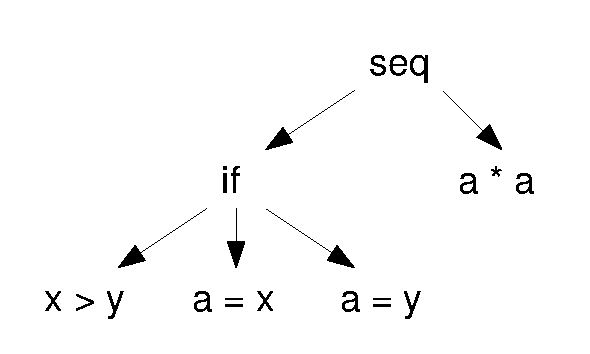
\includegraphics[scale=0.6]{instree.pdf}
  \caption{木構造をした命令}\label{fig:impl-instree}
 \end{center}
\end{minipage}
\begin{minipage}{0.5\hsize}
 \begin{center}
  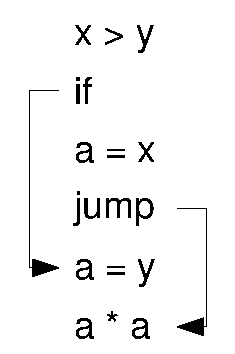
\includegraphics[scale=0.6]{insliner.pdf}
  \caption{直線化した命令}\label{fig:impl-insliner}
 \end{center}
\end{minipage}
\end{figure}
\end{resbonsiblesection}

\begin{resbonsiblesection}{生成するデータ構造}{\kobori}\label{sc:impl-data-structure}%正直位置が微妙
 実行時にメモリ上へ生成するデータ構造:タプルや配列,クロージャについて
 説明する.

\subsection{データ型の表現}
プログラム中のデータは大きく次の2通りに分かれる.
\begin{itemize}
 \item \typename{int}や\typename{float}などの基底型
 \item タプルや配列などの複合型
\end{itemize}

基底型は目的とする計算機に対して自然な表現を採用する.たとえば
\typename{int}型はマシンワード\footnote{ある計算機にとってもっとも扱いや
すいビット幅のこと.IA-32アーキテクチャならば32ビット幅となる.}と等しい
ビット幅を持ち``タグ''などが付加されることはない.また全て値型であり,直
接スタックやレジスタに置かれる.\typename{float}型には倍精度浮動小数点数
を採用した.これもスタックやレジスタに直接確保される.

タプルと配列はヘッダとして,長さやデータがポインタであるかを示すLayout
Bitmap\cite{Nguyen:2006:CMP:1140335.1140364}を持つ.これは,将来的にガベー
ジコレクタを実装する為に使用し,また比較演算の実装に用いる(詳しくは
\refSc{sc:impl-runtime}を参照のこと).

クロージャは先頭に関数のアドレス,続きに自由変数の値を持つタプルとして表
現される.ヴァリアントは型構築子を示す整数と後続にデータ本体を持つ``ドッ
トリスト''のように表現される.
\end{resbonsiblesection}

\begin{resbonsiblesection}{命令選択部}{\kobori}\label{sc:impl-inst}
 一旦,データを割付けるレジスタを決定しないままにIA-32アーキテクチャに存
 在する命令に仮想機械語を変換する.仮想機械語では独立したデスティネーショ
 ンオペランドを持つが,IA-32アーキテクチャでは2オペランドの片側が兼用に
 なっている命令が殆どである.元の値を保存する必要があるため,データの複
 製を行い,そのコピーに対して演算を行うようにした.

 一部の命令は使用できるレジスタが固定であるので,それはこの段階で割り当
 てることとした.それには呼び出し規約を満足させるために,戻り値を適切な
 レジスタに移動することも含む.

 また一部の命令に対しては,演算強度の低減に当たるような命令選択も行なっ
 ている.
\end{resbonsiblesection}

\begin{resbonsiblesection}{レジスタ割り当て}{\kobori}\label{sc:impl-regalloc}
 まず,末尾から走査することで,ある命令の実行時点で生存している一時変数の
 一覧を作成する.その後,上から飽食的に一時変数へレジスタを割り当ててい
 く.制御フローの合流地点においては,生存している変数を全てスタックフレー
 ム上に割り当てることで相互間でのレジスタの位置合せを軽減する.

 できる限り寿命となった変数の割り当てられたレジスタから優先的に使用する
 ことでレジスタ間転送を削減させる.

 レジスタ割り当てを実行し,スタックにスピルするデータを決定したことでス
 タックへ確保する駆動フレームのサイズと値の型がわかる.これを用い
 て,\lstinline|Entry|というスタブの位置にスタックフレームを確保する命令
 を挿入する.

 2011年2月3日時点,まだRegAllocモジュールは実装されていない.このため,
 現在出力できるアセンブリ言語ではレジスタ名のかわりに一時変数名が出力さ
 れる.
\end{resbonsiblesection}

\begin{resbonsiblesection}{実行時ランタイム}{\kobori}\label{sc:impl-runtime}
 実行時に必要となるライブラリには次のものがある.
\begin{itemize}
 \item メモリ管理機構
 \item 複合型に対する比較器
 \item エントリーポイントとなるmain関数
\end{itemize}
 
 2011年2月3日時点,実行時ランタイムとなるCプログラムは実装されていない.

\subsection{メモリ管理機構}
メモリ管理部は,プログラムの実行開始してすぐにタプルや配列を割付けるヒー
プを確保する.管理の都合から次の3種に分けて確保する.
\begin{itemize}
 \item 標準的なサイズのデータ\footnote{\typename{int}型以下のサイズを持
       つ値のことを指す.これにはポインタも含む.}を持つリスト領域
 \item 大きなサイズのデータ\footnote{\typename{float}型のことを指す.}を
       持つリスト領域
 \item その他,タプルと配列の領域
\end{itemize}

これに加え,標準的なサイズのデータのリスト領域に対しては,データ部がポイ
ンタであるかを示すbitmapを領域全体に対して用意する.

また,それぞれの領域に必要なだけメモリを確保するアロケータが必要である.
アロケータは確保したいデータの種類ごとに用意される.それぞれは必要なメモ
リ領域を引数に取るが,タプルや配列を確保するアロケータは,ヘッダ部分のメ
モリ領域を追加しただけのメモリを割り当てる.そして,ヘッダ領域は返される
ポインタより前の部分置く.こうしてポインタが直接データ本体を指すようにす
ることで,データアクセスを単純かつ高速になるようにする.

\subsection{複合型に対する比較器}
一般にポインタの内部を比較するとき,関数の特殊化の都合から内部のデータ構
造をコンパイル時に知ることができない.そのため,ヘッダ部分を見ながら比較
を行う関数を作成することとした.リストであるかどうかは,ポインタが指す領
域を比較することで判定ができる.タプルか配列であるかはヘッダの構造からわ
かる.ポインタかどうかも同様である.これらを使うことで同一であるかの判定
をすることができる.

\subsection{エントリーポイントとなる関数}
メモリ管理機構を起動し,トップレベル変数の束縛を順に行う関数を呼び出すエ
ントリーポイントとなる関数はC言語で作成する.
\end{resbonsiblesection}

\chapter{サンプルプログラムと実行結果}\label{ch:sample-program}

\chapter{結論}\label{ch:conclude}
我々は関数型言語に特徴的な機能,第一級の関数やクロージャ,型推論などの複
雑な機能を持つコンパイラ実装することで,それらに対する理解を深めるべく本
実験を実施した.
その方策として,MinCamlを見本に新たなコンパイラの実装を行った.これによっ
て,背景にある理論と計算機の表現力について多くの見識を得ることができた.

しかし,設計したコンパイラの実装を完成させるには至らなかった.これには次
の様な理由が考えられる.
\begin{itemize}
 \item 実装する機能の規模の見積りが甘かった
 \item 言語仕様の策定に時間を取られすぎた
 \item 両者とも経験の薄い環境での実装にしてしまった
 \item 理論の学習に対する手間を軽く考えすぎた
\end{itemize}

いずれともプロジェクト運営そのものの問題であり,自らの能力不足を痛感する
こととなった.これからの開発においては,工数などの見積りなど計画段階にお
いて,自らの能力と使うことのできる時間を考え適切な課題設定ができるよう反
省してこうと考える.

また,これからの時間を有効活用し,抜け落ちている機能や未実装の部分に取り
組み,現状の仕様のコンパイラの完成を目指したい.その後に,初期からの構想
である,
\begin{itemize}
 \item 多言語(C言語)との協調動作
 \item ごみ集めの実装
 \item マクロ機能などのメタプログラミング支援
 \item 分割コンパイル
\end{itemize}
なども考えていきたい.
\begin{flushright}[文責: 小堀 育男]\end{flushright}

%\chapter*{謝辞}
\addcontentsline{toc}{chapter}{謝辞}
\section*{謝辞}
樋口先生にはプロジェクト計画についてご意見をいただきました.大墳先生には発表
資料の作成や発表についてご指導いただきました.牛田先生には予稿などの書法につ
いて助言をいただきました.深謝の意を表します.

\bibliographystyle{jplain}
\bibliography{reference}

\backmatter
\appendix

\end{document}
